\documentclass[]{article}

\usepackage{amsmath}
\usepackage{graphicx}
\graphicspath{{images/}}
\usepackage{url}
\bibliographystyle{unsrt}
% opening
\title{Can Computer Think}
\author{Mohamed El. Kuku}

\begin{document}

\maketitle

\begin{abstract}
Recent advances in machine learning  have had a huge impact in AI. Thanks to the huge
amount of data available today, and the computations resources,
we are now able to obtain results that surpasses human experts in vision,
language, and even in some of the very difficult tasks such as radiology. That
also make ask question: have we built intelligent machines. This article
discusses current success in the field of deep learning, and try to understand
what makes a computer program, intelligent.
To the extent that most of use cases concerns, we can conclude that we have
built machines that are capable to do what it was designed for, achieving an
unprecedented level of intelligence. Though, we have not yet built a general
intelligent machines, and also no: Skynet is not coming any soon.
\end{abstract}

\section{What is Intelligence}

To answer this question, I believe, we first need to answer: what thinking really is. For decades, scientists were trying to mimic the human brain. And they failed. 

What is conscious? Does it define intelligence? Is there any secret recipe that
we are missing?\\

Deep learning is now the man of the show. It just magically works out of the
box. In recent ImageNet \cite{imagenet-competition} competition, CNN \cite{imagenet} has
achieved an accuracy that surpassed human. This is very big. In Go \cite{wiki:go}, an
ancient game, a machine learning algorithm was able to beat the best player in
the world in this game. Notice that Go is way too harder than chess game, for
start, there are $10^{170}$ board configurations--more than the number of atoms in
the known universe \cite{wiki:go}.\\

The bottom line is human do not need that such huge amount of data to e.g., play
well at go, or to know a cat just from one picture of it--and to generalize too.

\section{To Learn is To Generalize}

To learn is to generalize, is to tick into hidden layers searching for meanings.
In natural language processing, using not-even-deep networks such as word2vec
\cite{word2vec}, we were able to \textit{infer} relationship from our training,
that we did not ask the network to do. The learned word representations capture
meaningful semantics regularities in a very simple way. The regularities are
observed as a constant vector offset between pairs of words sharing a particular
relationship. If we denote the vector for word $i$ as $x_i$, and focus on the
singular/plural relation, we find that,
\begin{equation*}
  x_{family}-x_{families} \approx x_{car} - x_{cars}.
\end{equation*}

\subsection{Why BigData}
The brain is very efficient is using data. We are not. Our current algorithms
need tons of data to perform the most basic tasks in vision or language. A
toddler does not need to see thousands of pictures of a cat to recognize it.\\

There are two paths: the engineers, practitioners path, and the scientists or
philosophical path. The former needs just immediate results, the later however,
needs to dig even more, to understand how things work the way they do. Research
depends on funding--which is becoming ever harder. We need to digest the
basics. But not organization prefers direct applicable results. That is probably
why researchers like Yoshua Bengio preferred not to work to any corporation. And
that is why also, Geoffrey Hinton launched his Vector institute to do basic
research in machine learning.

\section{Artificial General Intelligence}
This is a long term research goal. We are currently rely on supervised learning
to build our models. Supervised learning needs training data--which makes its
inference only local to this data, up-to some extent. To fix that, the obvious
way is to use the opposite of our underlying model, to use unsupervised
learning. Unfortunately, unsupervised learning is not as successful as it
sibling is. Transfer learning might be our best shot so far. But it is definitely
not the solution. There is some interesting phenomena in our brain that allows
it to easily achieve intelligence, and understand relationship.


\subsection{What are we missing}
Several years ago, before 2012 Alex's \cite{imagenet} model, deep learning was
there. The reason why deep learning was not as dominant as the case now, is
basically because we had not had that much of data, nor that much of
computational resources (GPUs). Alex model was indeed a breakthrough, but since
then there was not as much breakthrough (maybe except for GAN \cite{gan}).\\

Have we reached the intrinsic limitations of our current algorithms. That might be correct,
which also suggest why prominent researchers like Hinton suggests to rethink about the
whole back-propagation thing \cite{wiki:hinton}. In Figure
\ref{fig:space-ml}, shows the parameter space of current machine learning
research. Ironically, lots of breakthrough in machine learning happens because
of hyper-parameters tuning--we tinker them to find the best configurations. In this case, we only have three parameters to tune
such that we find the best configurations. The dataset is no longer the issue,
even in historically known secret field like biology research, we now have
access to freely available dataset. The computing resources is also not the
problem. Thanks to nVidia and AWS one can scale to whatever extent they like
(assuming that the funding is available). The only left parameter is the
algorithm. Well, that is both good and bad. At least we do not have scary
parameters to try and tune. We only just have one. The problem is, the
underlying theory behind deep learning (and machine learning) consists of
statistics and probabilities, optimization, calculus, linear algebra, in
addition to computer science field. That means we basically need to go through
so many fields to solve this problem. 
\begin{figure}
  \centering
  \label{fig:space-ml}
  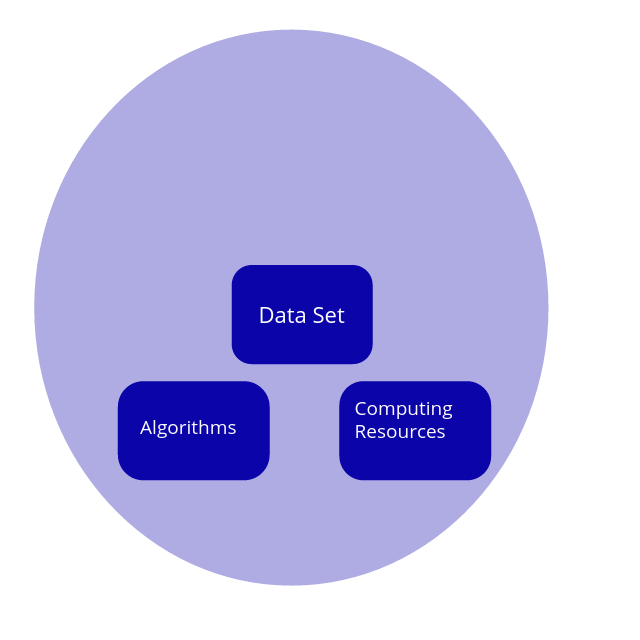
\includegraphics[scale=0.3]{image}
  \caption{The current (hyper)parameters in machine learning practice. Now, we
    have lots of data, and access to even lots of resources computing. But we
    still lack in the algorithms part. Algorithms are difficult to develop, they
  are lifetime research, however their impact is really huge. Big players in
  machine learning, and hence AI, are the big tech companies. They just need
  direct results. They need to plug this \textit{`AI'} in their cameras and social
  apps. The bright side however, is that their competition is what drives the
  current very fast pace of machine learning research.}
\end{figure}

\section{What Next}
We have achieved huge success in many aspects of Artificial Intelligence. This
should not be forgotten. It is also good and
healthy that the deep learning community has variety of diversity: people are coming
from all kind of fields and give their contributions and their unique
perspective. Having both theory oriented, and production-ready researchers
is good as well, in that we can get the benefit from the two worlds.\\

The answer of this question, whether we will ever have intelligent machines,
will lead us to unprecedented quest. That will question our own intelligence,
our feelings, and everything we once thought is human. Perhaps we are missing the
\textit{Rosetta Stone}, or perhaps intelligence is just deep layers that uses
weights to make decision. We are on the edge of something very big. Something
fundamental that will challenge all of our pre-knowledge--all of our believes
and thoughts. It will hit very hard, but the pay-off will be huge. We will, in
any case, get to know what are we better than ever before. \\

For me, as a machine learning researcher and practitioner, it is a lifetime
research topic. I think, we should use artificial intelligence to help
\textit{us} understand how our brains work, not the other way around. This
research of understanding what intelligence is will lead me to a quest
To the extent that most of our AI use cases concern, we can happily rely on our
current AI technology. We cannot however say that, these machines are
intelligent. We need to figure out what intelligence really is, first. The
current research path led us to unprecedented results, but basic research, is
important.

\bibliography{reference}

\end{document}
